\documentclass[t,aspectratio=169, 8pt]{beamer}
\usetheme{baurg}
\usepackage{rg-code-beamer}

\usepackage[english]{babel}
\usepackage{subcaption}
% Maths and Physics
\usepackage{amsmath}
\usepackage{amsthm}
\usepackage{amssymb}
\usepackage{physics}
\usepackage{tabularx}
\usepackage{braket}
\usepackage{bm}
\usepackage{array,multirow,graphicx}


\def\*#1{\bm{#1}}

% For figures
\usepackage{tikz}
\usetikzlibrary{decorations.pathmorphing}
\usetikzlibrary{shapes}
\usetikzlibrary{matrix,shapes.geometric}
\usetikzlibrary{positioning,fit,calc} 
\usepackage{svg}
\usepackage{subcaption}

% set size of code in minted environments
\setsize{small}

\title{Solvatochromic Shifts in the Spectroscopy of Acetone}
\subtitle{\Large with LAMMPS and VOTCA}
\author{August 13, 2021}
\department{LAMMPS Virtual Workshop 2021}

\begin{document}

\begin{titleframe}[variant=1,bgimage=background.png]
\end{titleframe}

\begin{chapterframe}
  \frametitle{Overview}
  \begin{itemize}
    \item How to follow along
    \item The QM/MM Approach
    \item Doing QM/MM with LAMMPS AND VOTCA
  \end{itemize}
\end{chapterframe}


%%%%%%%%%%%%%%%%%%%%%%%%%%%%%%%%%%%%%%%%%%%%%%%%%%%%%%%%%%%%%%%%%%%%%%%%%%%%%%%
% SETUP OF THE TUTORIAL
%%%%%%%%%%%%%%%%%%%%%%%%%%%%%%%%%%%%%%%%%%%%%%%%%%%%%%%%%%%%%%%%%%%%%%%%%%%%%%%%

\begin{frame}[fragile]
  \frametitle{How to follow along}
  You can follow along with this tutorial on you own pc. If you use the VM of the LAMMPS tutorial, docker will already be installed, otherwise you can install it (Ubuntu)
  \begin{minted}{bash}
sudo apt install docker.io
  \end{minted}
  and pull the votca image.
  \begin{minted}{bash}
docker pull votca/votca
  \end{minted}
  Next we start docker and load the environment variables of VOTCA
  \begin{minted}{bash}
docker run -it votca/votca /bin/bash
source VOTCARC.bash
  \end{minted}
  To get all the necessary input files
  \begin{minted}{bash}
git clone https://github.com/rubengerritsen/lammps
cd lammps
\end{minted}
  Now you are all set to follow along.
\end{frame}


%%%%%%%%%%%%%%%%%%%%%%%%%%%%%%%%%%%%%%%%%%%%%%%%%%%%%%%%%%%%%%%%%%%%%%%%%%%%%%%
% THE QMMM APPROACH
%%%%%%%%%%%%%%%%%%%%%%%%%%%%%%%%%%%%%%%%%%%%%%%%%%%%%%%%%%%%%%%%%%%%%%%%%%%%%%%%
\begin{frame}
  \frametitle{The QM/MM Approach}
  \centering
  \includegraphics[height=0.65\textheight]{images/siteenergies}
\end{frame}

\begin{frame}
  \frametitle{The QM/MM Approach: A combination of 4 models}
  \begin{columns}[t]
    \begin{column}{0.44\textwidth}
      \begin{itemize}
        \item Molecular Dynamics:
              \begin{itemize}
                \item Used to obtain a snap shot of the topology of the molecular system
                \item \textbf{Tool:} LAMMPS (or GROMACS)
                \item \textbf{Representation:} Geometry + Forcefield
              \end{itemize}
        \item Quantum Mechanical:
              \begin{itemize}
                \item Used to compute the excited states of a molecule and generate input files.
                \item \textbf{Tool:} VOTCA (excited states) + ORCA (input files)
                \item \textbf{Representation:} Optimized geometry
              \end{itemize}
      \end{itemize}
    \end{column}
    \begin{column}{0.44\textwidth}
      \begin{itemize}
        \item Electrostatics:
              \begin{itemize}
                \item The electrostatics are computed based on a multipole expansion (in this tutorial just partial charges).
                \item \textbf{Tool:} VOTCA (and ORCA)
                \item \textbf{Representation:} Distributed multipoles
              \end{itemize}
        \item Polarization:
              \begin{itemize}
                \item We use the applequist model with Thole damping, i.e. polarizable dipoles.
                \item \textbf{Tool:} VOTCA (and ORCA)
                \item \textbf{Representation:} Distributed polarizabilities
              \end{itemize}
      \end{itemize}
    \end{column}
  \end{columns}
  \vspace{0.5cm}
  To do a QM/MM calculation we need to setup the representations for each model and generate all the necessary input files.
\end{frame}


%%%%%%%%%%%%%%%%%%%%%%%%%%%%%%%%%%%%%%%%%%%%%%%%%%%%%%%%%%%%%%%%%%%%%%%%%%%%%%%%
% QMMM WITH VOTCA
%%%%%%%%%%%%%%%%%%%%%%%%%%%%%%%%%%%%%%%%%%%%%%%%%%%%%%%%%%%%%%%%%%%%%%%%%%%%%%%%
\begin{chapterframe}
  \frametitle{Performing QM/MM with VOTCA and LAMMPS}
  The process of performing a QM/MM calculation consists of three general steps.
  \begin{enumerate}
    \item Create representations and input files
    \item The mapping procedure (combining the representations from the 4 models)
    \item Running the QM/MM calculation
  \end{enumerate}
\end{chapterframe}

\begin{frame}[fragile]
  \frametitle{The System and Generating Input Files}
  \begin{columns}[b]
    \begin{column}{0.58\textwidth}
      \textbf{The MD trajectory of Acetone in Water}\\
      The MD trajectory can be obtained by running a normal LAMMPS simulation of your system. For this tutorial we have already performed the MD simulation for you. The relevant data can be found in the \mintinline{bash}{system.data} and \mintinline{bash}{traj1.dump} files.
      \vspace{0.3cm}\\
      \textbf{Optimized geometries}\\
      Optimized geometries can be obtained from many QM packages including VOTCA. For this tutorial we have already computed them with ORCA. The ORCA results and the input files that generated them can be found in the \mintinline{bash}{DFT_ORCA} folder.
      \vspace{0.3cm}\\
      \textbf{Multipoles and Polarization}\\
      The multipoles and polarization can also be computed with ORCA and that is what we did for this tutorial.The ORCA output files, however, need to be converted to a VOTCA readable format called mps files.
    \end{column}
    \begin{column}{0.4\textwidth}
      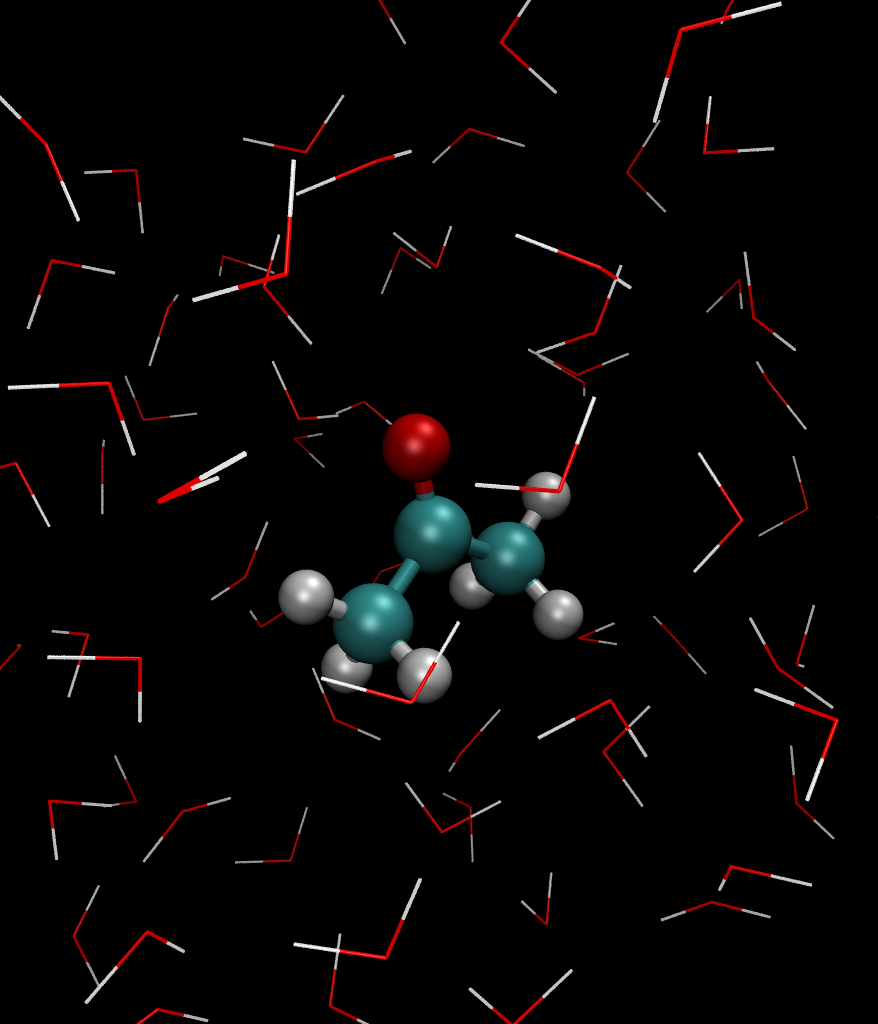
\includegraphics[width=0.95\textwidth]{system}
    \end{column}
  \end{columns}
\end{frame}

\begin{frame}[fragile]
  \frametitle{Generating the Multipole and Polarizability files}
  For the multipoles and polarization VOTCA uses mps files. There is a special tool in VOTCA that converts ORCA log files with CHELPG charges to an mps file.
  \begin{minted}{bash}
xtp_tools -e log2mps -o OPTIONS/log2mps_water.xml
  \end{minted}
  We see here the typical way of calling a VOTCA program
  \begin{minted}{bash}
xtp_<executableType> -e <calculationType> -o <optionsFile>.xml
  \end{minted}
  The option file
  \begin{minted}{xml}
<options>
    <log2mps>
        <dftpackage>orca</dftpackage>
        <input>DFT_ORCA/water/chelpg.log</input>
        <output>MP_FILES/water_n.mps</output>
    </log2mps>
</options>
  \end{minted}
\end{frame}

\begin{frame}[fragile]
  \frametitle{How to find out which options are available?}
  \begin{enumerate}
    \item Look at the description of a program with the describe flag \mintinline{bash}{-d}\\
          \begin{minted}{bash}
xtp_tools -d log2mps
    \end{minted}
    \item Print (\mintinline{bash}{-p}) an example options file with \textbf{all} available options to an output file (\mintinline{bash}{-o})
          \begin{minted}{bash}
xtp_tools -p log2mps -o optionsLog2mps.xml
    \end{minted}
  \end{enumerate}
\end{frame}


\begin{frame}[fragile]
  \frametitle{The result of \textit{log2mps}}
  The generated MPS file.
  \begin{minted}{text}
! GENERATED BY VOTCA::XTP::::LOG2MPS 
! N=3 Q[e]=+0.0000000
Units angstrom
  O +0.0000000 +0.0000000 -0.0043320 Rank 0
    -0.7585550
    P +0.8370000
  H +0.7614610 +0.0000000 +0.5795250 Rank 0
    +0.3787500
    P +0.4960000
  H -0.7614610 +0.0000000 +0.5795250 Rank 0
    +0.3798050
    P +0.4960000
  \end{minted}
  But the polarizations are still wrong!
\end{frame}

\begin{frame}[fragile]
  \frametitle{Fitting Polarizabilities}
  To obtain the atomic polarizabilities we fit them such that they represent the
  molecular polarizabillity as close as possible. The molecular polarizabilities
  are calculated with ORCA for this tutorial. VOTCA has a tool specifically for
  this fitting procedure.
  \begin{minted}{bash}
xtp_tools -e molpol -o OPTIONS/molpol_water.xml
  \end{minted}
  The options file
  \begin{minted}{xml}
<options>
  <molpol>
    <input>MP_FILES/water_n.mps</input>
    <output>MP_FILES/water_n_pol.mps</output>
    <mode>qmpackage</mode>
    <qmpackage>orca</qmpackage>
    <logfile>DFT_ORCA/water/chelpg.log</logfile>
  </molpol>
</options>
  \end{minted}
  Check the output file.
\end{frame}

\begin{frame}[fragile]
  \frametitle{Repeat for the Acetone molecule}
  To generate the mps file for acetone
  \begin{minted}{bash}
xtp_tools -e log2mps -o OPTIONS/log2mps_acetone.xml
xtp_tools -e molpol -o OPTIONS/molpol_acetone.xml
  \end{minted}

\end{frame}


%%%%%%%%%%%%%%%%%%%%%%%%%%%%%%%%%%%%%%%%%%%%%%%%%%%%%%%%%%%%%%%%%%%%%%%%%%%%%%%%
% MAPPING 
%%%%%%%%%%%%%%%%%%%%%%%%%%%%%%%%%%%%%%%%%%%%%%%%%%%%%%%%%%%%%%%%%%%%%%%%%%%%%%%%
\begin{frame}[fragile]
  \frametitle{The Mapping Procedure: An Example}
  \setsize{footnotesize}
  \begin{minted}{xml}
<mdatoms>1:O223:0 1:C222:1 1:C80:2 1:C80:3 1:H85:4 1:H85:5 1:H85:6 1:H85:7 1:H85:8 1:H85:9</mdatoms>
<qmatoms>0:O      1:C      2:C     3:C     4:H     5:H     6:H     7:H     8:H     9:H</qmatoms>
<mpoles>0:O       1:C      2:C     3:C     4:H     5:H     6:H     7:H     8:H     9:H</mpoles>
<localframe>0 1 3</localframe>
  \end{minted}
  \setsize{small}

  \begin{center}
    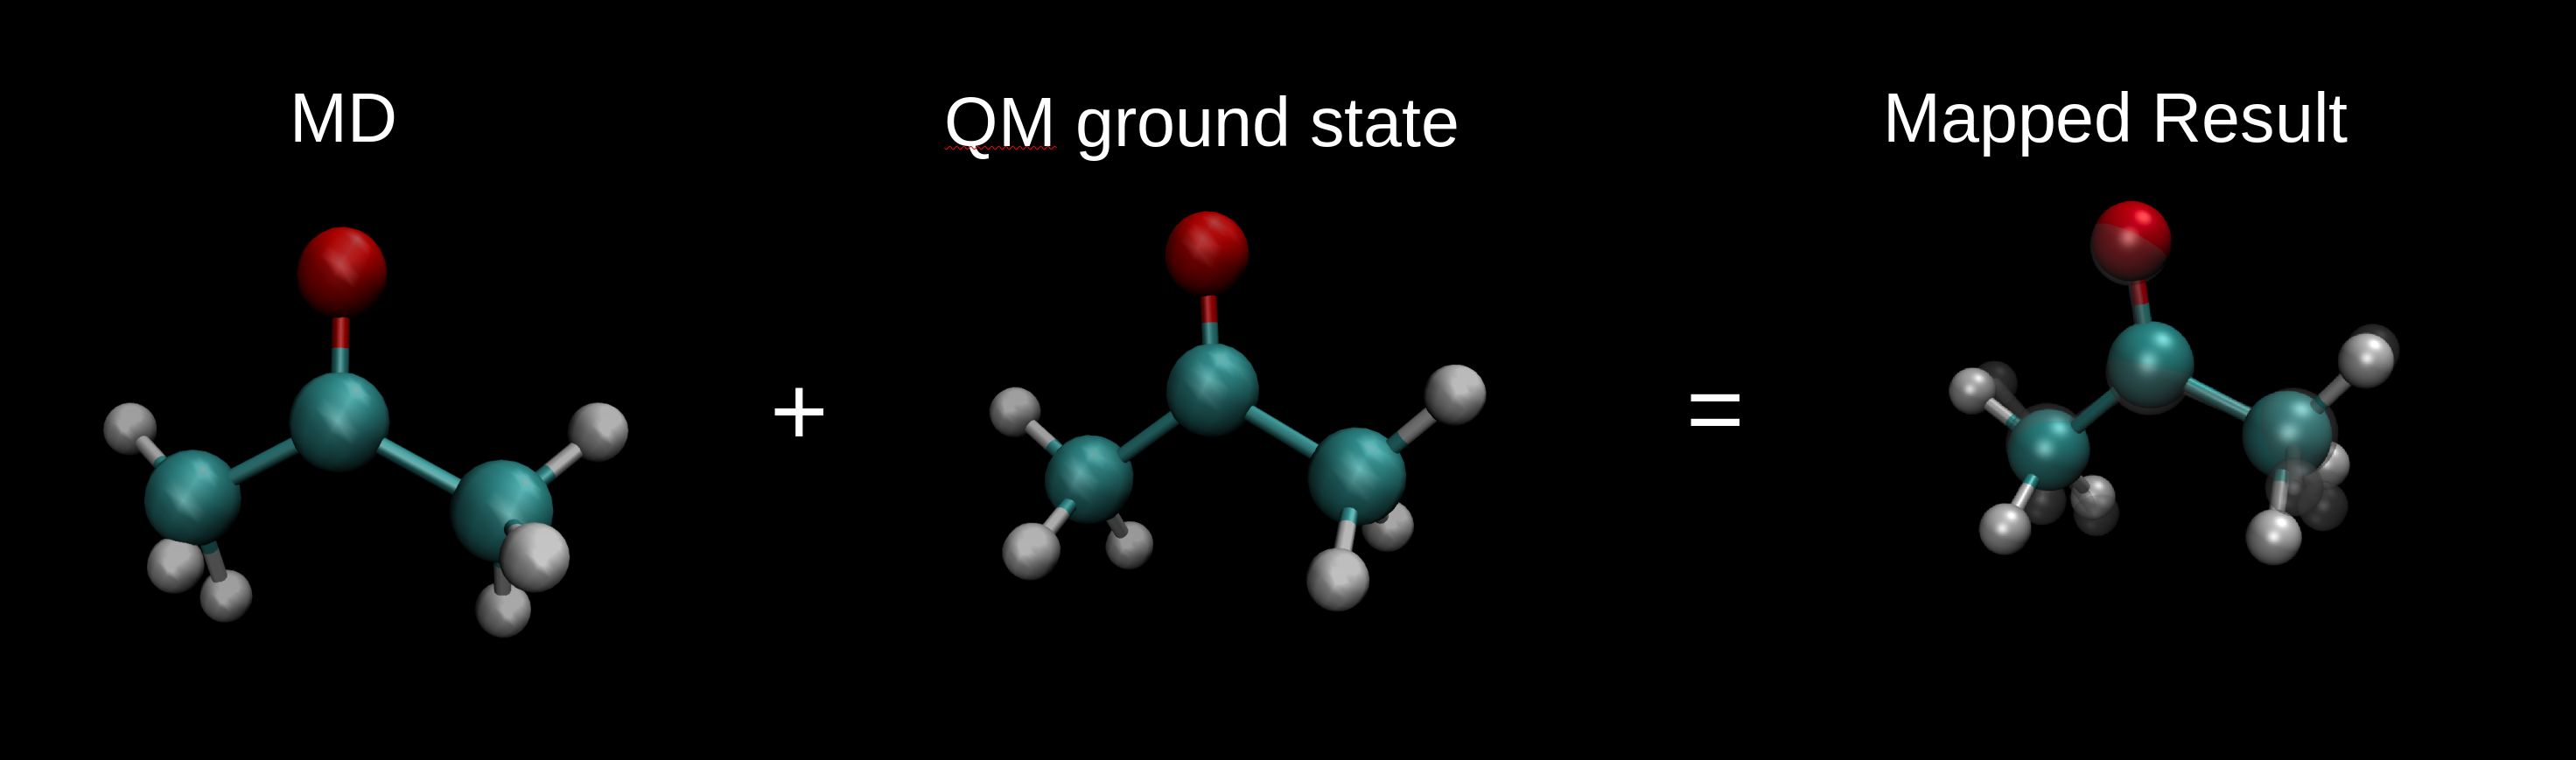
\includegraphics[width=0.8\textwidth]{images/mdAndqm/mapping}
  \end{center}

  \small This procedure needs to be done for every
  \begin{itemize}
    \item geometry (i.e. optimized QM geometry or multipole geometry)
    \item and for every molecule
  \end{itemize}
\end{frame}

\begin{frame}[fragile]
  \frametitle{The Mapping Procedure: The Mapping File}
  \setsize{footnotesize}

  \begin{minted}{xml}
<molecule>
  <mdname>C3H6O1</mdname>
  <segments>
    <segment>
      <name>ACETONE</name>
      <qmcoords_n>DFT_ORCA/acetone/acetoneOpt.xyz</qmcoords_n>
      <qmcoords_e>DFT_ORCA/acetone/acetoneOpt.xyz</qmcoords_e>
      <qmcoords_h>DFT_ORCA/acetone/acetoneOpt.xyz</qmcoords_h>
      <multipoles_n>MP_FILES/acetone_n_pol.mps</multipoles_n>
      <map2md>0</map2md>
      <fragments>
        <fragment>
          <name>acetone</name>
          <mdatoms>1:O223:0 1:C222:1 1:C80:2 1:C80:3 1:H85:4 1:H85:5 1:H85:6 1:H85:7 1:H85:8 1:H85:9</mdatoms>
          <qmatoms>0:O 1:C 2:C 3:C 4:H 5:H 6:H 7:H 8:H 9:H</qmatoms>
          <mpoles>0:O 1:C 2:C 3:C 4:H 5:H 6:H 7:H 8:H 9:H</mpoles>
          <weights>16 12 12 12 1 1 1 1 1 1</weights>
          <localframe>0 1 3</localframe>
        </fragment>
      </fragments>
    </segment>
  </segments>
</molecule>
  \end{minted}
\end{frame}

\begin{frame}[fragile]
  \frametitle{The Mapping Procedure: Performing and Checking the Mapping}
  \setsize{footnotesize}
  Once the mapping file is setup, performing the mapping is easy.

  \begin{minted}{bash}
xtp_map -t LAMMPS/system.data -c LAMMPS/traj1.dump -s OPTIONS/mapping.xml -f state.hdf5
  \end{minted}

  To check what the mapping did we can print pdb files with the original coordinates and the multipole or qm coordinates to visually check (e.g. in VMD) if the mapping procedure was successful. To run the map checker
  \begin{minted}{bash}
xtp_run -e mapchecker -o OPTIONS/mapchecker.xml -f state.hdf5
  \end{minted}
  In the option file you can specify exactly which states and configurations you would like to check.
\end{frame}

%%%%%%%%%%%%%%%%%%%%%%%%%%%%%%%%%%%%%%%%%%%%%%%%%%%%%%%%%%%%%%%%%%%%%%%%%%%%%%%%
% Setup of Job File
%%%%%%%%%%%%%%%%%%%%%%%%%%%%%%%%%%%%%%%%%%%%%%%%%%%%%%%%%%%%%%%%%%%%%%%%%%%%%%%%
\begin{frame}[fragile]
  \frametitle{Setup the QM/MM jobfile and run the calculation}
  \setsize{footnotesize}
  To perform the QM/MM calculation we need a jobfile that describes for which molecule(s) and which state(s) the calculation is performed. 
\setsize{footnotesize}
  \begin{minted}{xml}
<io_jobfile>
  <states>n s1</states>
  <segments>0 1</segments>
  <use_gs_for_ex>true</use_gs_for_ex>
</io_jobfile>
  \end{minted}
  To create the jobfile
  \begin{minted}{bash}
xtp_parallel -e qmmm -o OPTIONS/qmmm.xml -f state.hdf5 -j "write"
  \end{minted}
  Running is easy
  \begin{minted}{bash}
xtp_parallel -e qmmm -o OPTIONS/qmmm.xml -f state.hdf5 -j "run" -x 6
  \end{minted}
  Read the results from the output file and store them in \mintinline{bash}{state.hdf5}.
  \begin{minted}{bash}
xtp_parallel -e qmmm -o OPTIONS/qmmm.xml -f state.hdf5 -j "read"
  \end{minted}

\end{frame}

%%%%%%%%%%%%%%%%%%%%%%%%%%%%%%%%%%%%%%%%%%%%%%%%%%%%%%%%%%%%%%%%%%%%%%%%%%%%%%%%
% Results
%%%%%%%%%%%%%%%%%%%%%%%%%%%%%%%%%%%%%%%%%%%%%%%%%%%%%%%%%%%%%%%%%%%%%%%%%%%%%%%%
\begin{frame}[fragile]
  \frametitle{Basic results}
  The results of the QM/MM calculation can be found in the \mintinline{bash}{qmmm_jobs.xml} file.
  \vspace{0.1cm}\\
  Every job has a new \mintinline{bash}{<output>} section where the computed energies can be found.
  \setsize{footnotesize}
  \begin{minted}{xml}
<output>
  <regions>
    <region Tot_charge="-3.200000e+01" id="0" size="1" type="qmregion">
      <E_total>-5252.342575</E_total>
    </region>
    <region Tot_charge="0.000000e+00" id="1" size="101" type="polarregion">
      <E_static>-30.978427</E_static>
      <E_polar>-9.246523</E_polar>
      <E_total>-40.224950</E_total>
    </region>
  </regions>
  <E_tot>-5292.567526</E_tot>
  <Compute_Time>24</Compute_Time>
  <Total_Charge>-32.000000</Total_Charge>
  <Iterations>4</Iterations>
</output>
  \end{minted}
\small
NB. Only energy differences make sense here, hence to get the energy of the first singlet level we compute the difference between the total energy of the singlet job with the total energy of the groundstate, i.e. $\Omega_S = E_S - E_n$.
\end{frame}


\begin{chapterframe}
  \frametitle{More advanced results: the density of states}
  \begin{columns}[c]
    \begin{column}{0.48\textwidth}
      To determine the density of states we can perform a QM/MM calculation for
      many configurations. \\ \vspace{0.3cm} The picture on the right shows the
      density of states for the lowest energy singlet of acetone, computed for
      110 configurations, and the vaccuum level as a reference.
    \end{column}
    \begin{column}{0.48\textwidth}
      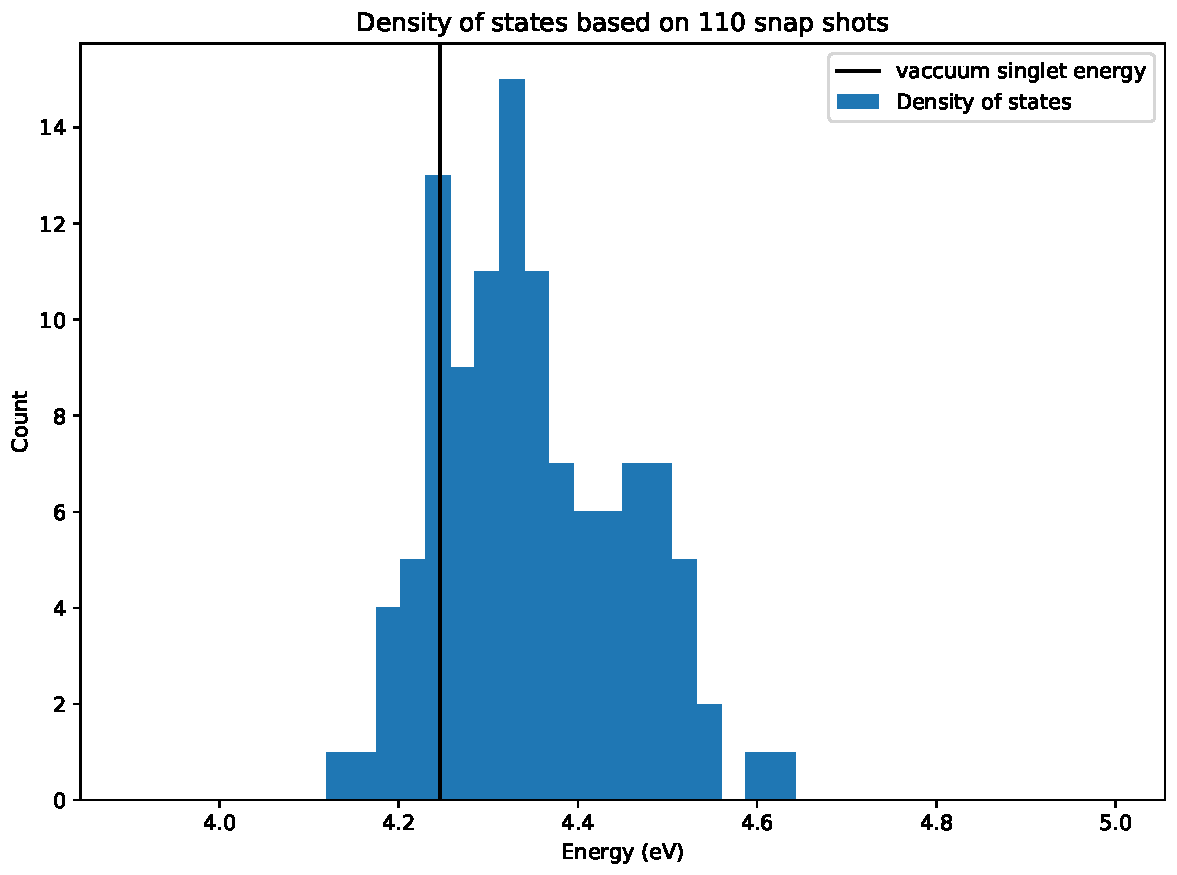
\includegraphics[width=0.95\textwidth]{images/dos/DOS_shifted.pdf}
    \end{column}
  \end{columns}
\end{chapterframe}

\title{Questions}
\begin{chapterframe}
	\frametitle{ ~}
	\vspace{1.5cm}
	\begin{center}
		{\fontsize{28}{48} \selectfont \bfseries{The End}}
	\end{center}
\end{chapterframe}


\end{document}